\FloatBarrier
\section{Seamless Streaming}\label{app:streaming}




















\subsection{Efficient Monotonic Multihead Attention}
\subsubsection{Definition of operators}
\label{app:streaming_operators}
\begin{table}[h]
    \centering
    \small
    \begin{tabular}{l|l|l}
    \toprule 
    Notation & Definition & PyTorch \\
    \midrule
    $A_{i,j}$ & Index $i$-th row and $j$-th column in matrix $A$ & \texttt{A[i, j]}\\
    $A_{i,:}$ & Index $i$-th row of $A$ as a vector& \texttt{A[[i], :]}  \\
    $A_{:,j}$ & Index $j$-th column of $A$ as a vector & \texttt{A[:, [j]]}\\
    $A \odot B$ & Element-wise product (Hadamard roduct) & \texttt{A * B} \\
    $A B$ & Matrix multiplication & \texttt{torch.bmm(A, B)} \\
    $\texttt{comprod}_l$(A) & Cumulative product on the $l$-th dimension & \texttt{torch.cumprod(A, dim=l)} \\
    $\texttt{comsum}_l$(A) & Cumulative summation on the $l$-th dimension & \texttt{torch.cumsum(A, dim=l)} \\
    $\texttt{triu}_b$(A) & Upper triangle of $A$ with a offset of $b$& \texttt{torch.triu(A, diagonal=b)} \\
    $J_{N\times M}$ & A matrix with size of $N$ by $M$, filled with 1 & \texttt{torch.ones(N, M)} \\
    $\texttt{roll}_k$ & Shift matrix by $k$ elements, on last dimension & \texttt{A.roll(k, dims=[-1])} \\
    \bottomrule
    \end{tabular}
    \caption{Matrix operations and their implementation in PyTorch.
    }
    \label{tab:emma_notations}
\end{table}

\subsubsection{Detailed derivation}
\label{app:emma_estimation}
Intuitively, the $\alpha$ can be estimated from dynamic programming:
\begin{equation}
    \alpha_{i,j} = p_{i,j} \sum_{k=1}^j \alpha_{i-1, k} \prod_{l=k}^{j-1}(1 - p_{i,l})
    \label{eq:alpha_orig}
\end{equation}

While 
\citep{raffel_online_2017}
gave a close form and parallel estimation of alignment,
the denominator in the equation can cause instability and alignment to vanish in the training.
We rewrite \Cref{eq:alpha_orig} as 
\begin{equation}
    \alpha_{i,:} = p_{i,:} \odot \alpha_{i-1, :} \mathrm{T}(i)  
\end{equation}
Where $\mathrm{T}(i)$ a transition matrix and each of its element:
\begin{equation}
    \mathrm{T}(i)_{m,n} =
    \begin{cases}
    \prod_{l=m}^{n-1} (1 - p_{i,l}) & m < n\\
    1 & m = n\\
    0 & m > n \\
    \end{cases}
\end{equation}
$\mathrm{T}(i)_{m,n}$ is the probability of the model reading from $x_m$ to $x_n$ with $y_{i}$ without writing.
Denote $t^{i}_{m,n} = \prod_{l=m}^{n} (1 - p_{i,l}) $
We can see that if we manage to have $\mathrm{T}(i)$, then the
$\alpha_{i, :}$ can be computed through matrix multiplication.

Define the probability from jumping from $x_m$ to $x_n$ with our write a new token $y_i$:

then we can define $\mathrm{T}(i)$ as
\begin{equation}
    \mathrm{T}(i) = \begin{pmatrix}
1 & t^{i}_{1,2} & t^{i}_{1,3} & t^{i}_{1,4}  &... & & t^{i}_{1,|X|}\\\
0 & 1 & t^{i}_{2,3} & t^{i}_{2,4} &... & & t^{i}_{2,|X|}\\
0 & 0 & 1 & t^{i}_{3,4} &... & & t^{i}_{3,|X|}\\
\vdots & \vdots & \vdots & \vdots  & & & \vdots \\
0 & 0 & 0 & 0 &... & & 1\\
\end{pmatrix}_{|X| \times |X|}
\end{equation}
It can be further expressed as
\begin{align}
    \mathrm{T}(i) &=
     \texttt{triu}_0 \left(\begin{pmatrix}
1 & t^{i}_{1,2} & t^{i}_{1,3} & t^{i}_{1,4}  &... & & t^{i}_{1,|X|}\\\
1 & 1 & t^{i}_{2,3} & t^{i}_{2,4} &... & & t^{i}_{2,|X|}\\
1 & 1 & 1 & t^{i}_{3,4} &... & & t^{i}_{3,|X|}\\
\vdots & \vdots & \vdots & \vdots  & & & \vdots \\
1 & 1 & 1 & 1 &... & & 1\\
\end{pmatrix}_{|X| \times |X|} \right)\\
&= \texttt{triu}_0\left(\texttt{cumprod}_2(1 - \mathrm{P}^{ext}(i))\right)
\end{align}
where $\texttt{triu}_b\left(\cdot\right)$
is a function to extract the upper triangle of a matrix with an offset $b$ \footnote{See $\texttt{torch.triu}$},
and $\texttt{cumprod}_2$ means that the computation is along the second dimension.
Additionally, the extended probably matrix $\mathrm{P}_i^{ext}$ is defined as
\begin{align}
    \mathrm{P}^{ext}(i)  &= \begin{pmatrix}
0 & p_{i,1} & p_{i,2}& ... & p_{i,|X| - 1}\\
0 & 0 & p_{i,2}& ... & p_{i,|X| - 1}\\
0 & 0 & 0& ... & p_{i,|X| - 1}\\
\vdots & \vdots & \vdots & & \vdots\\
0 & 0& 0& ... & p_{i,|X| - 1}\\
0 & 0& 0& ... & 0\\
\end{pmatrix}_{|X| \times |X|}\\
    &= \texttt{triu}_1 \left( \begin{pmatrix} 1 \\ \vdots \\ 1 \end{pmatrix}_{|X| \times 1}  \begin{pmatrix} p_{i,|X|} &p_{i,1} & ... & p_{i,|X| - 1} \end{pmatrix}_{1 \times |X|}\right)\\
    &= \texttt{triu}_1\left( J_{|X| \times 1} \texttt{roll}_1(p_{i,:})\right)
\end{align}
Where $J_{|X| \times 1}$ is an all one matrix with a size of $|X|$ by 1,
\footnote{$J_{|X| \times 1} \texttt{roll}_1(p_{i,:})$ can be achived by $\texttt{torch.expand}$ function.}
and $\texttt{roll}_k$ is the function shift matrix by $k$ elements \footnote{See \texttt{torch.roll}}.

In summary, we can rewrite \Cref{eq:alpha_orig} as
\begin{equation}
    \alpha_{i,:} = p_{i,:} \odot \alpha_{i, :} \texttt{triu}_0\left(\texttt{cumprod}_2(1 - \texttt{triu}_1\left( J_{|X| \times 1} \texttt{roll}_1(p_{i,:}) \right))\right)
\end{equation}

A code snippet of the implementation of EMMA in PyTorch is shown as follows: 
\begin{verbatim}

def monotonic_alignment(p):
    bsz, tgt_len, src_len = p.size()

    # Extension probablity matrix
    p_ext = p.roll(1, [-1]).unsqueeze(-2).expand(-1, -1, src_len, -1).triu(1)

    # Transition matrix
    T = (1 - p_ext).comprod(-1).triu()

    alpha = [p[:, [0]] * T[:, [0]]

    for i in range(1, tgt_len):
        alpha.append(p[:, [i]] * torch.bmm(alpha[i - 1], T[:, i]))
        
    return torch.cat(alpha[1:], dim=1)


\end{verbatim}

\subsection{Model Performance}
\begin{figure}[!ht]
    \centering
    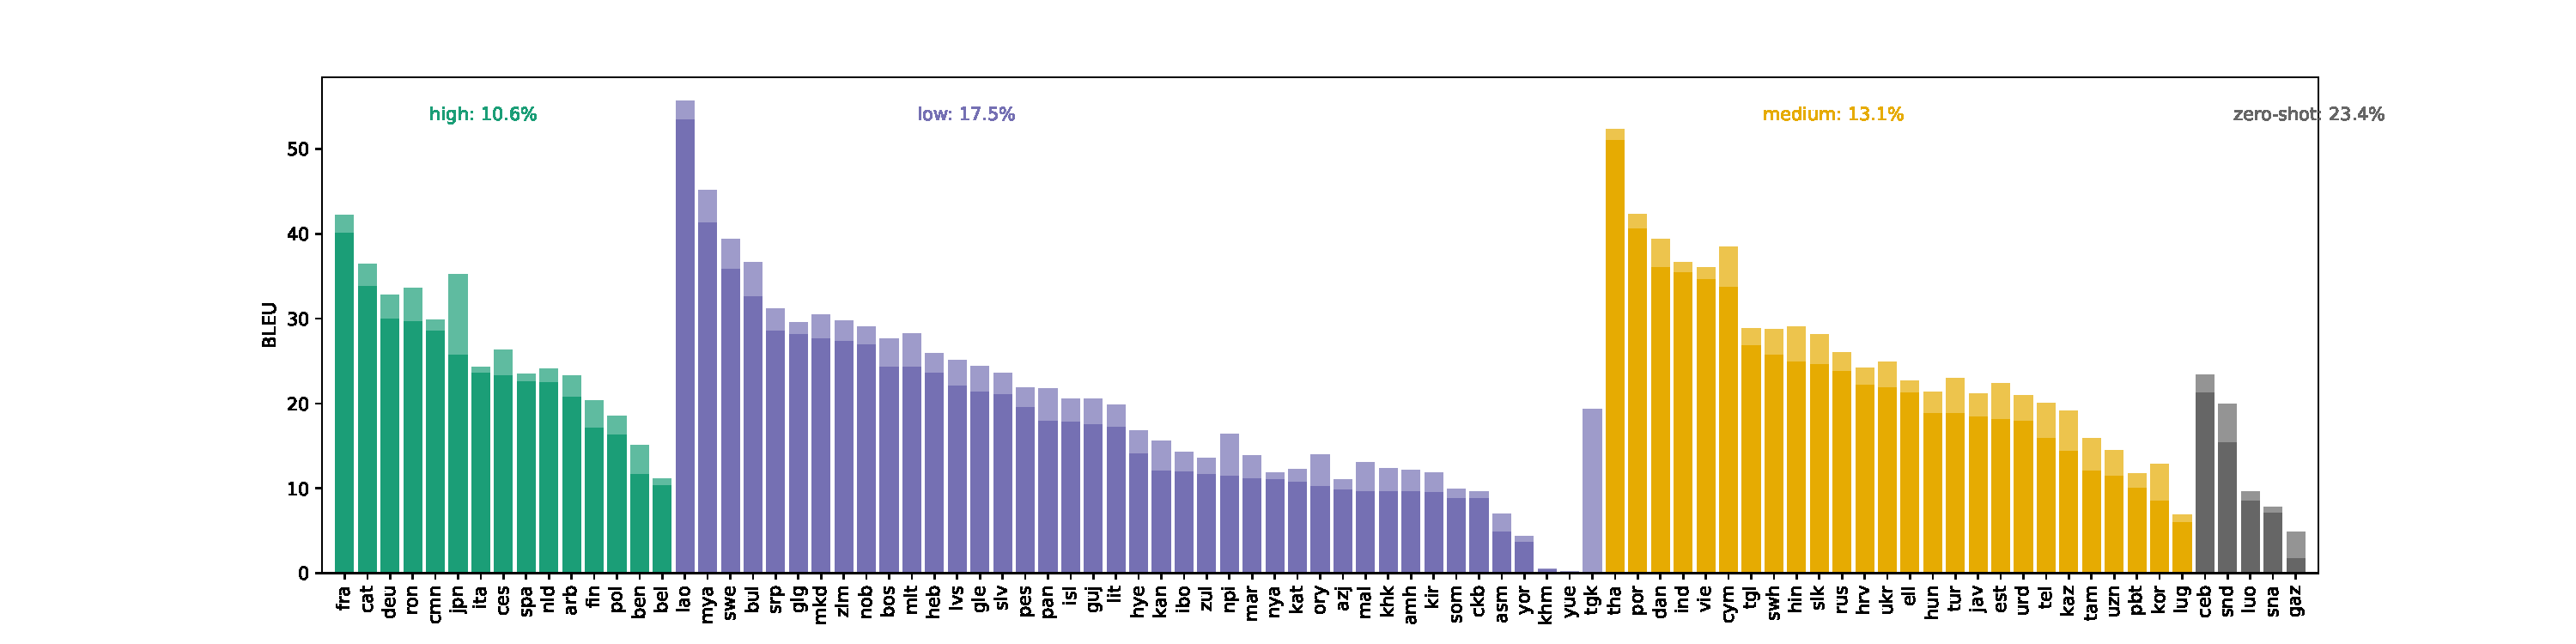
\includegraphics[width=1.0\textwidth]{figures/streaming/resources/ENG_X-BLEU.pdf}
    \caption{BLEU score of \seamlessstreaming compared with \mfourttwo, on \fleurs S2TT, \engx.}
\end{figure}
\begin{figure}[!ht]
    \centering
    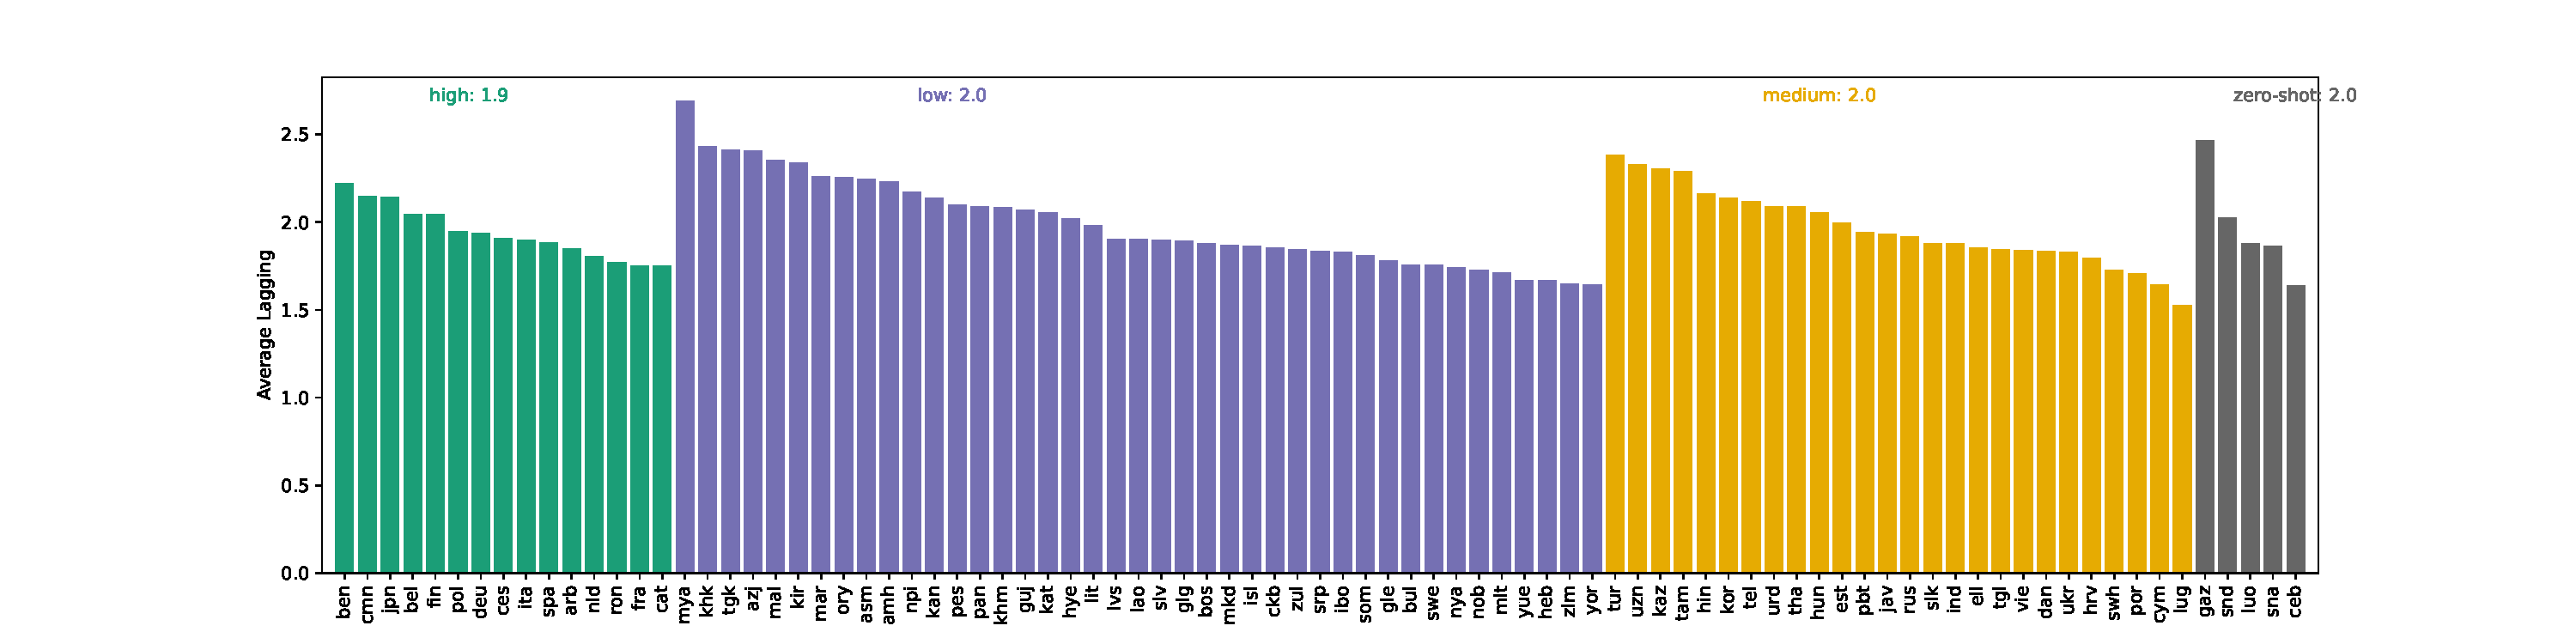
\includegraphics[width=1.0\textwidth]{figures/streaming/resources/ENG_X-AL.pdf}
    \caption{Latency of \seamlessstreaming on \fleurs S2TT, \engx.}
\end{figure}
\begin{figure}[!ht]
    \centering
    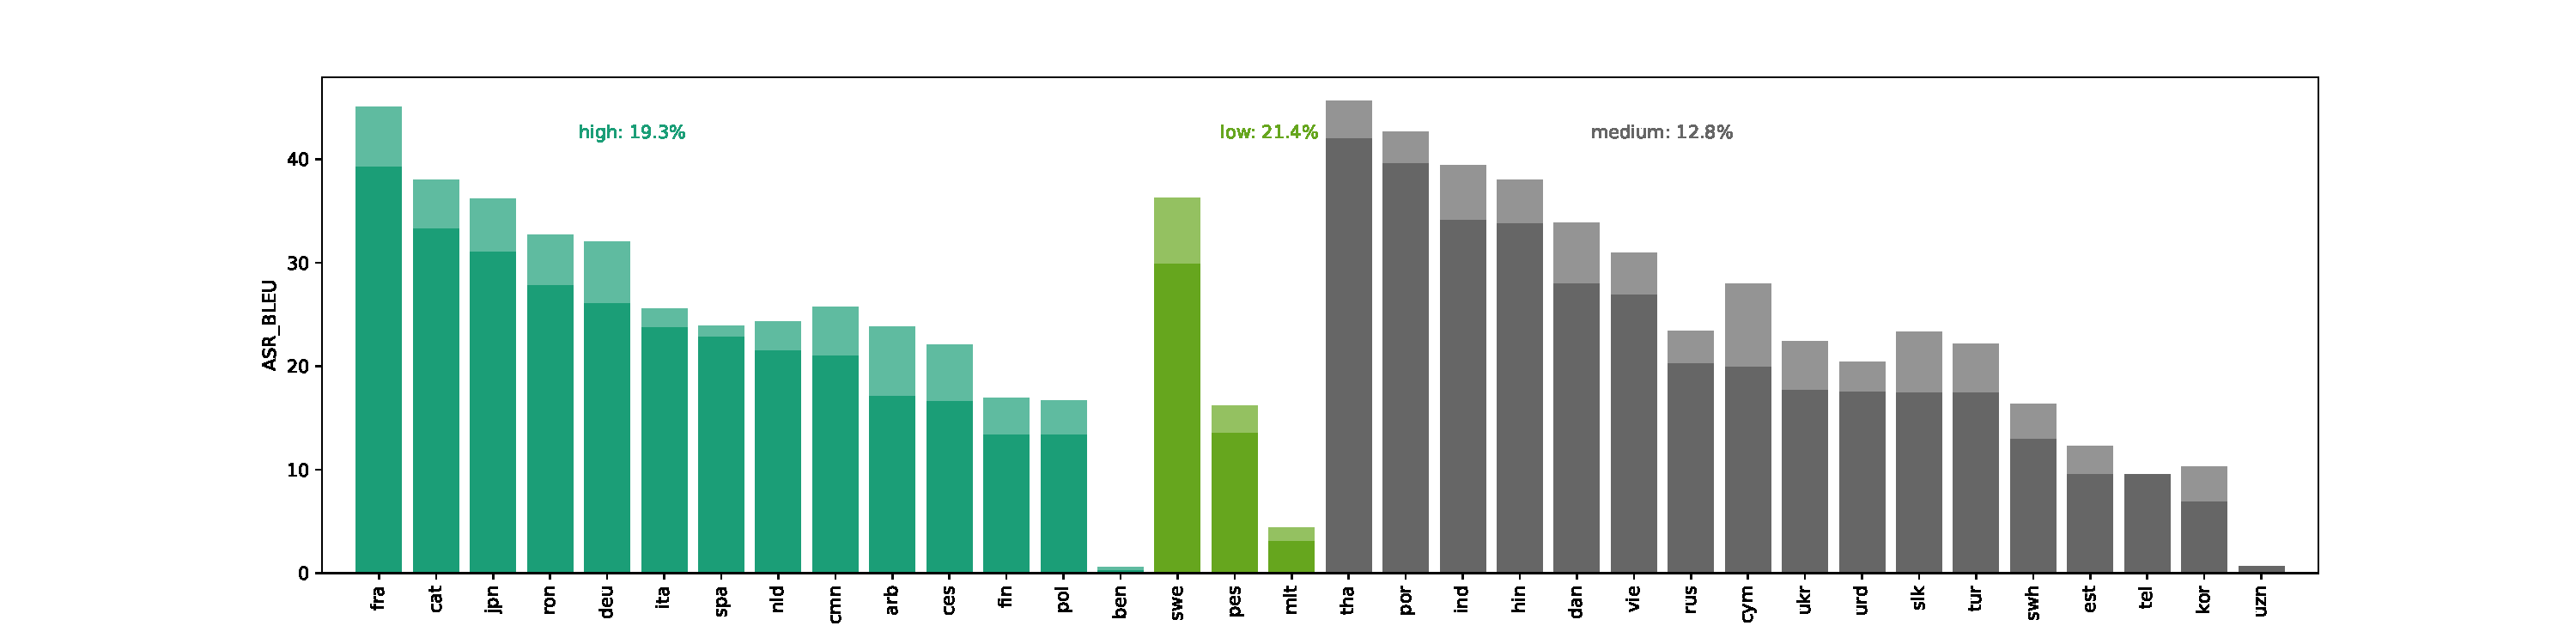
\includegraphics[width=1.0\textwidth]{figures/streaming/resources/ENG_X-SEAMLESS_WHISPER_ASR_BLEU.pdf}
    \caption{BLEU score of \seamlessstreaming, compared with \mfourttwo, on \fleurs S2ST, \engx.}
\end{figure}
\begin{figure}[!ht]
    \centering
    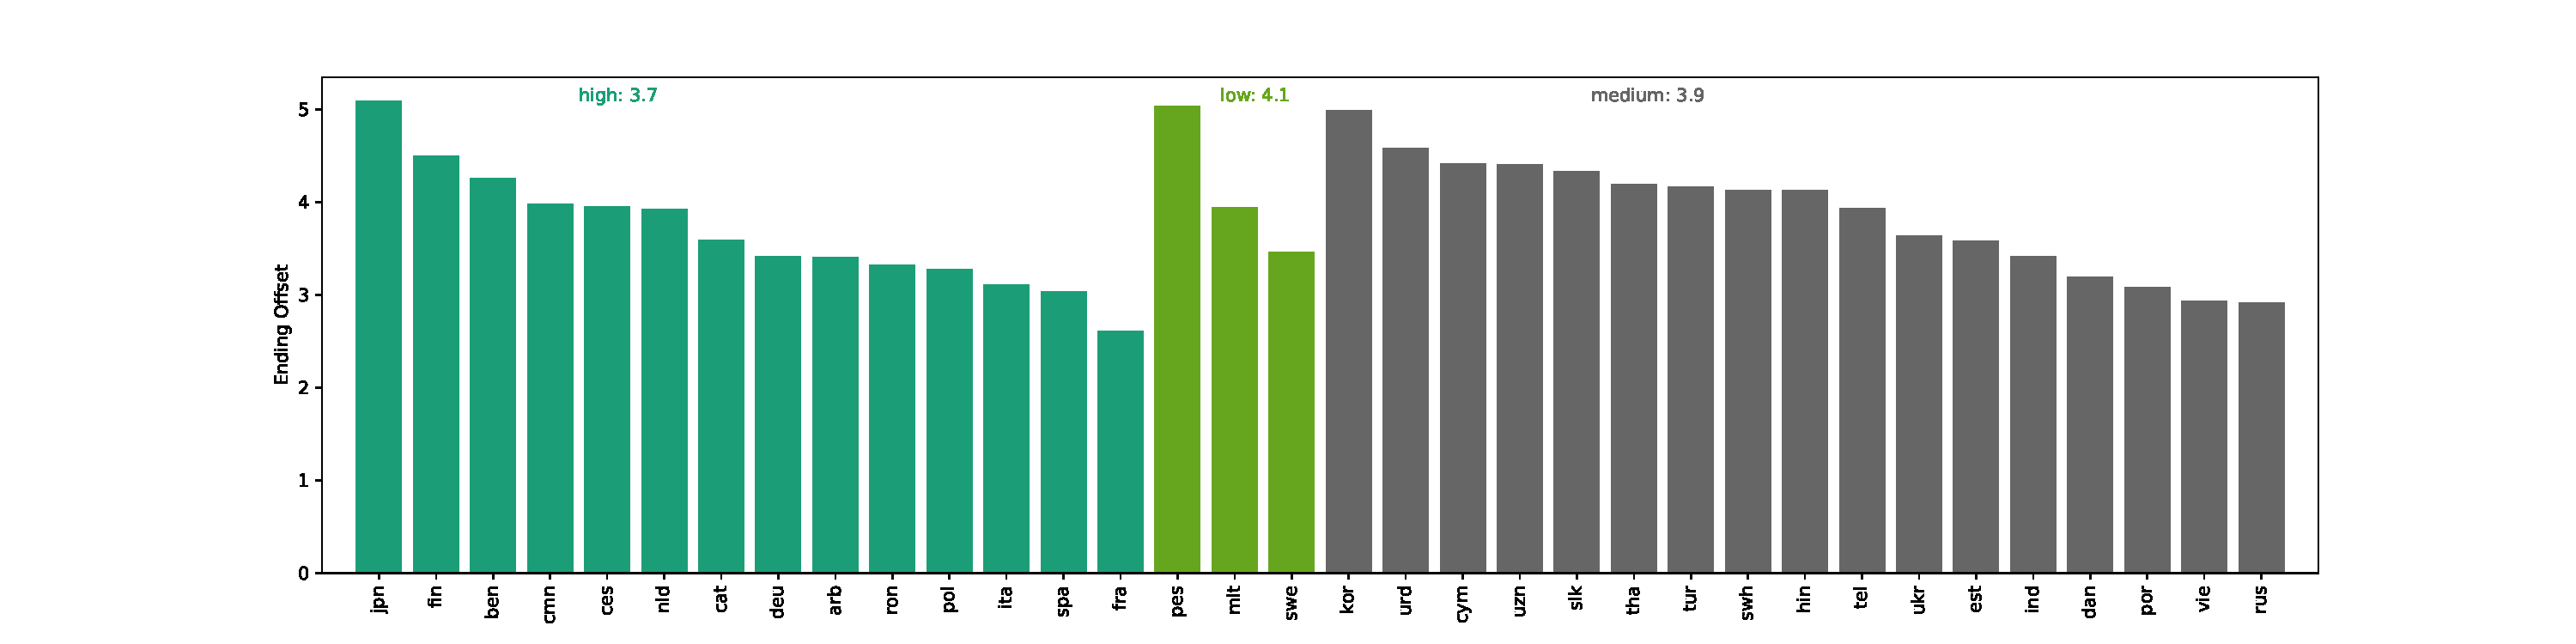
\includegraphics[width=1.0\textwidth]{figures/streaming/resources/ENG_X-EndOffset.pdf}
    \caption{Latency of \seamlessstreaming on \fleurs S2ST, \engx.}
\end{figure}
\begin{figure}[!ht]
    \centering
    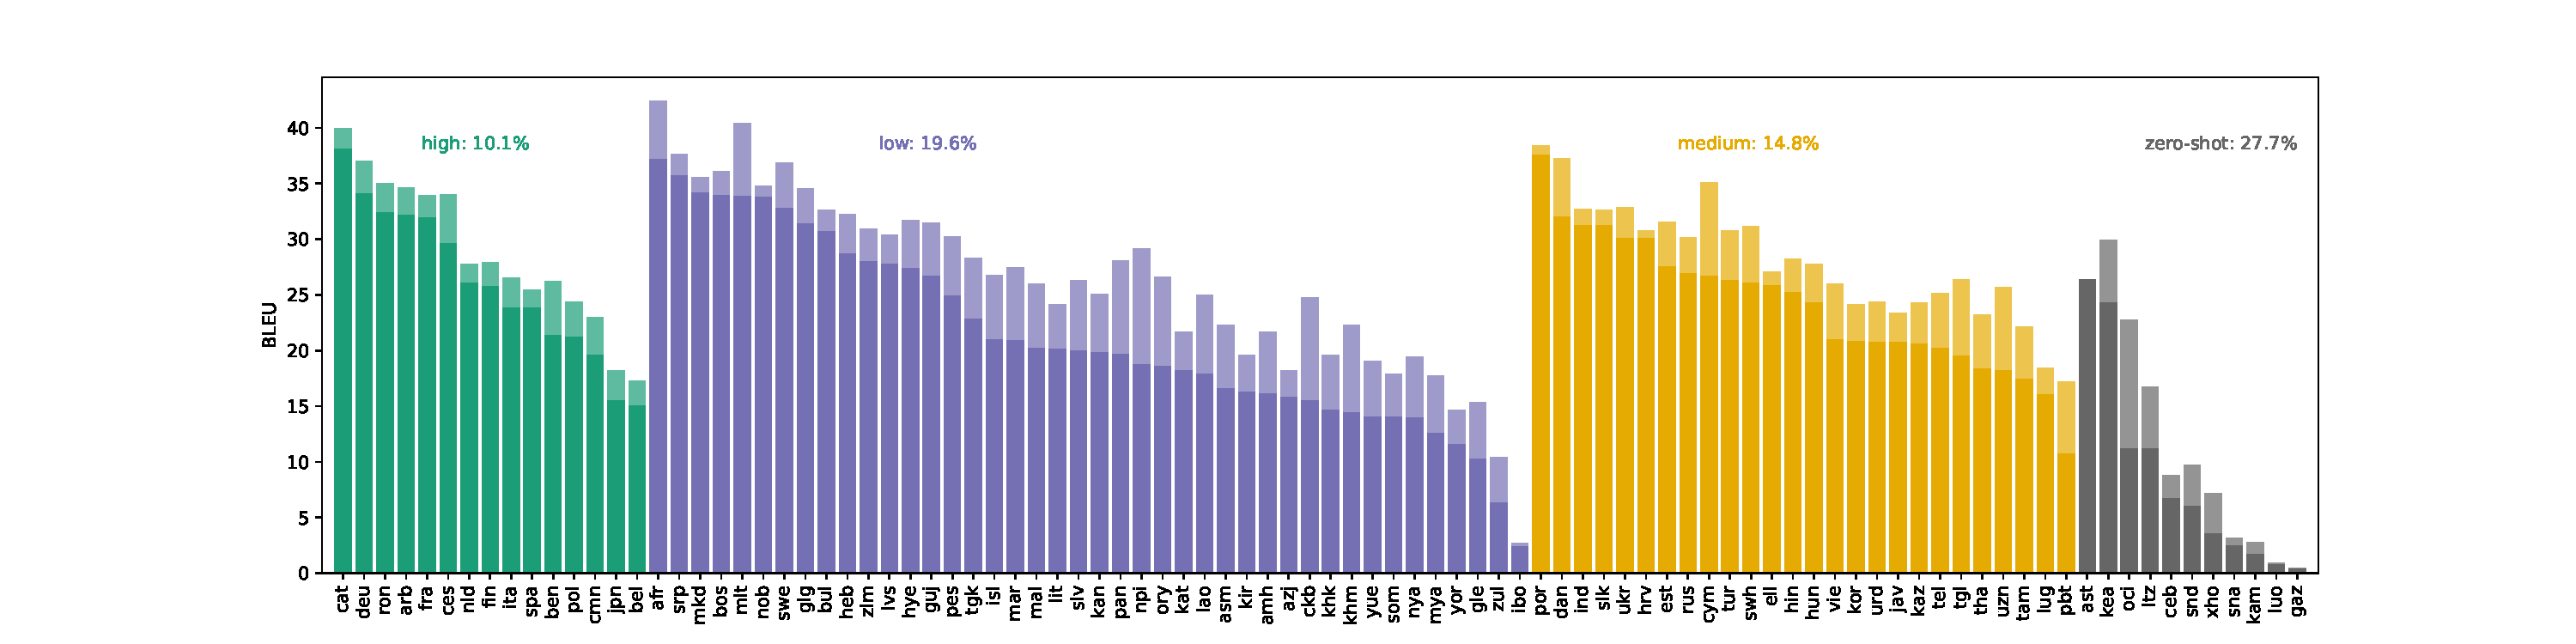
\includegraphics[width=1.0\textwidth]{figures/streaming/resources/X_ENG-BLEU.pdf}
    \caption{BLEU score of \seamlessstreaming compared with \mfourttwo, on \fleurs S2TT, \xeng.}
\end{figure}
\begin{figure}[!ht]
    \centering
    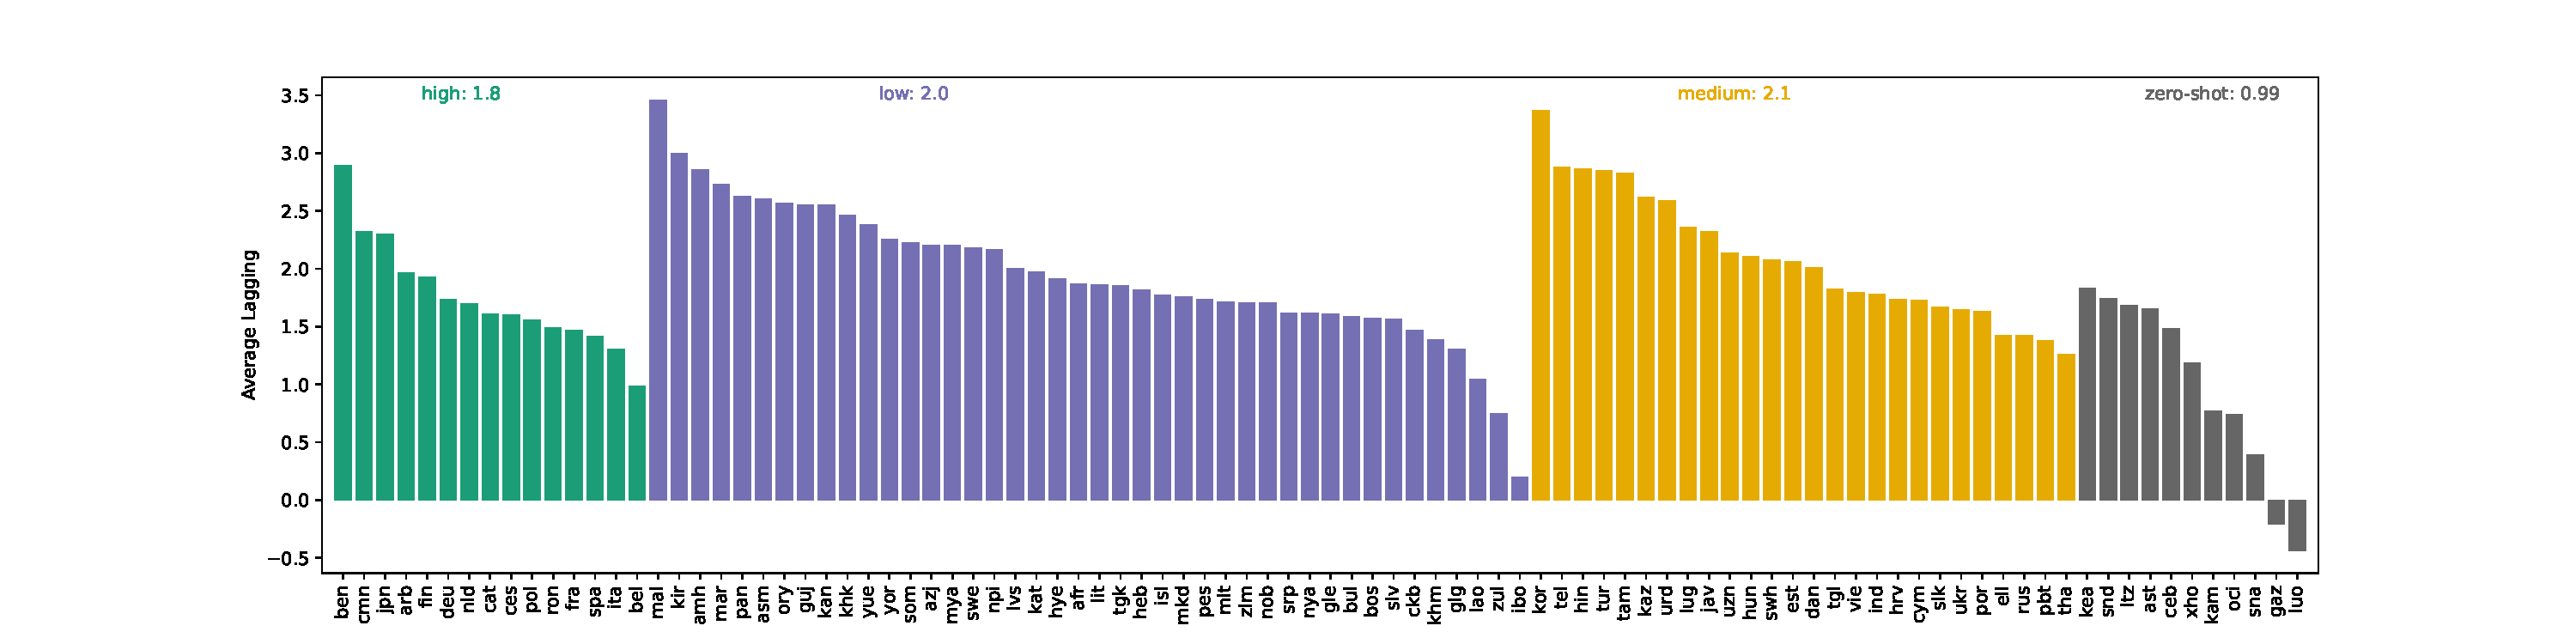
\includegraphics[width=1.0\textwidth]{figures/streaming/resources/X_ENG-AL.pdf}
    \caption{Latency of \seamlessstreaming on \fleurs S2TT, \xeng.}
\end{figure}
\begin{figure}[!ht]
    \centering
    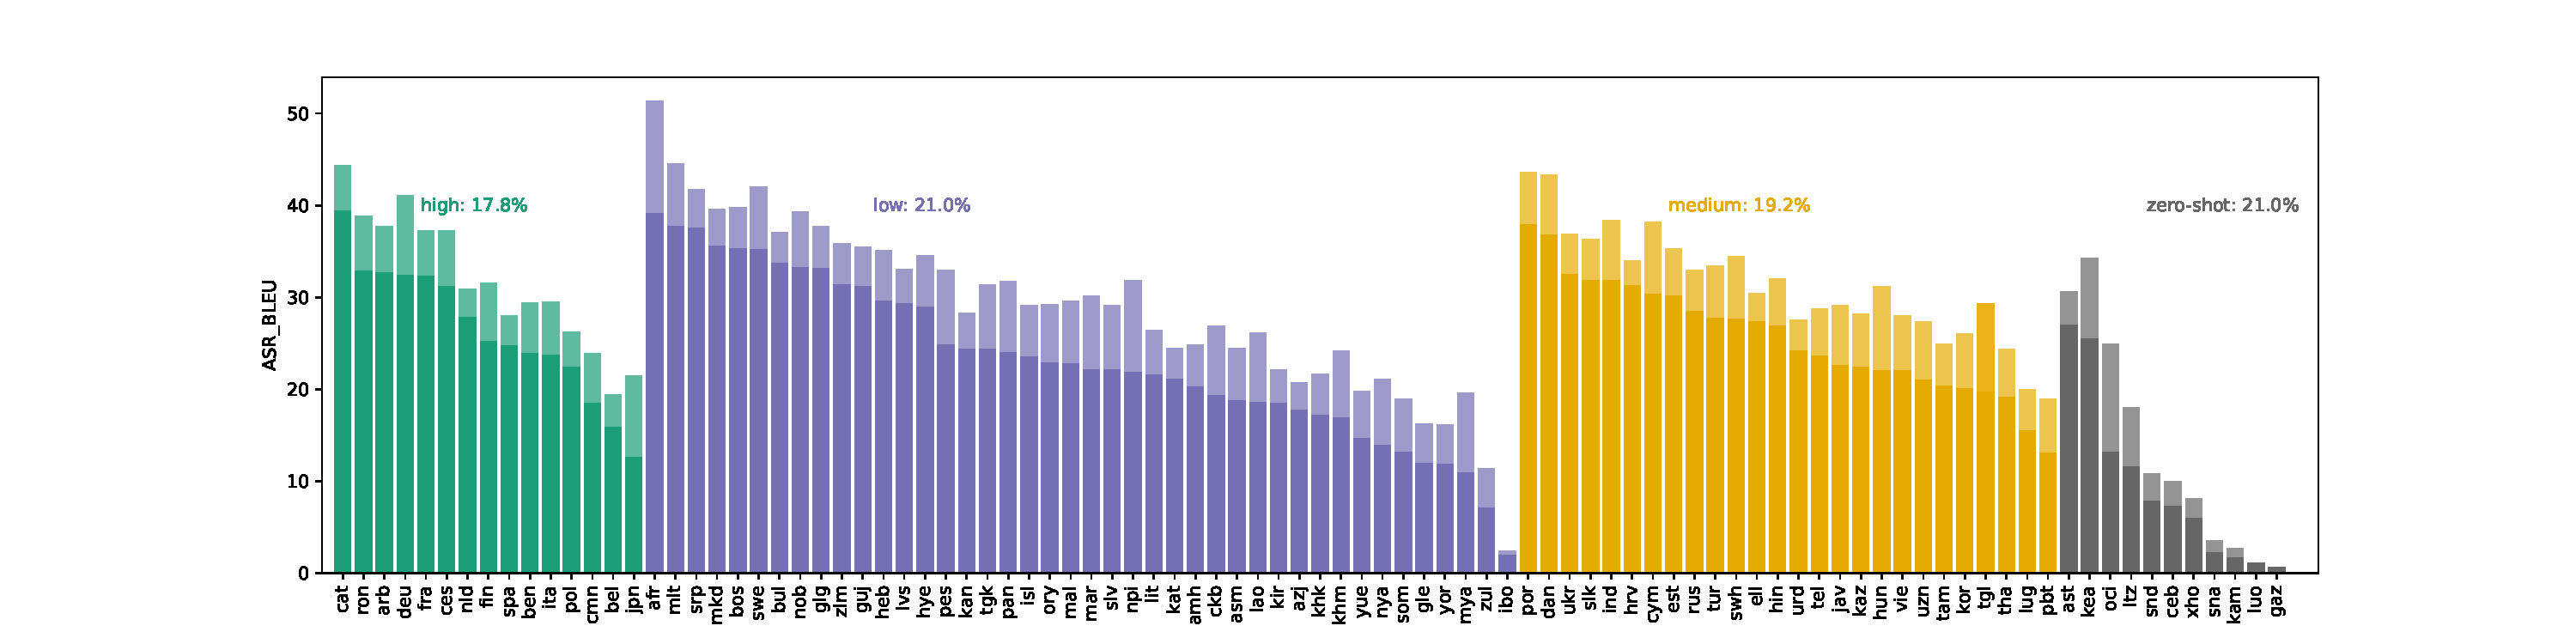
\includegraphics[width=1.0\textwidth]{figures/streaming/resources/X_ENG-SEAMLESS_WHISPER_ASR_BLEU.pdf}
    \caption{BLEU score of \seamlessstreaming, compared with \mfourttwo, on \fleurs S2ST, \xeng.}
\end{figure}
\begin{figure}[!ht]
    \centering
    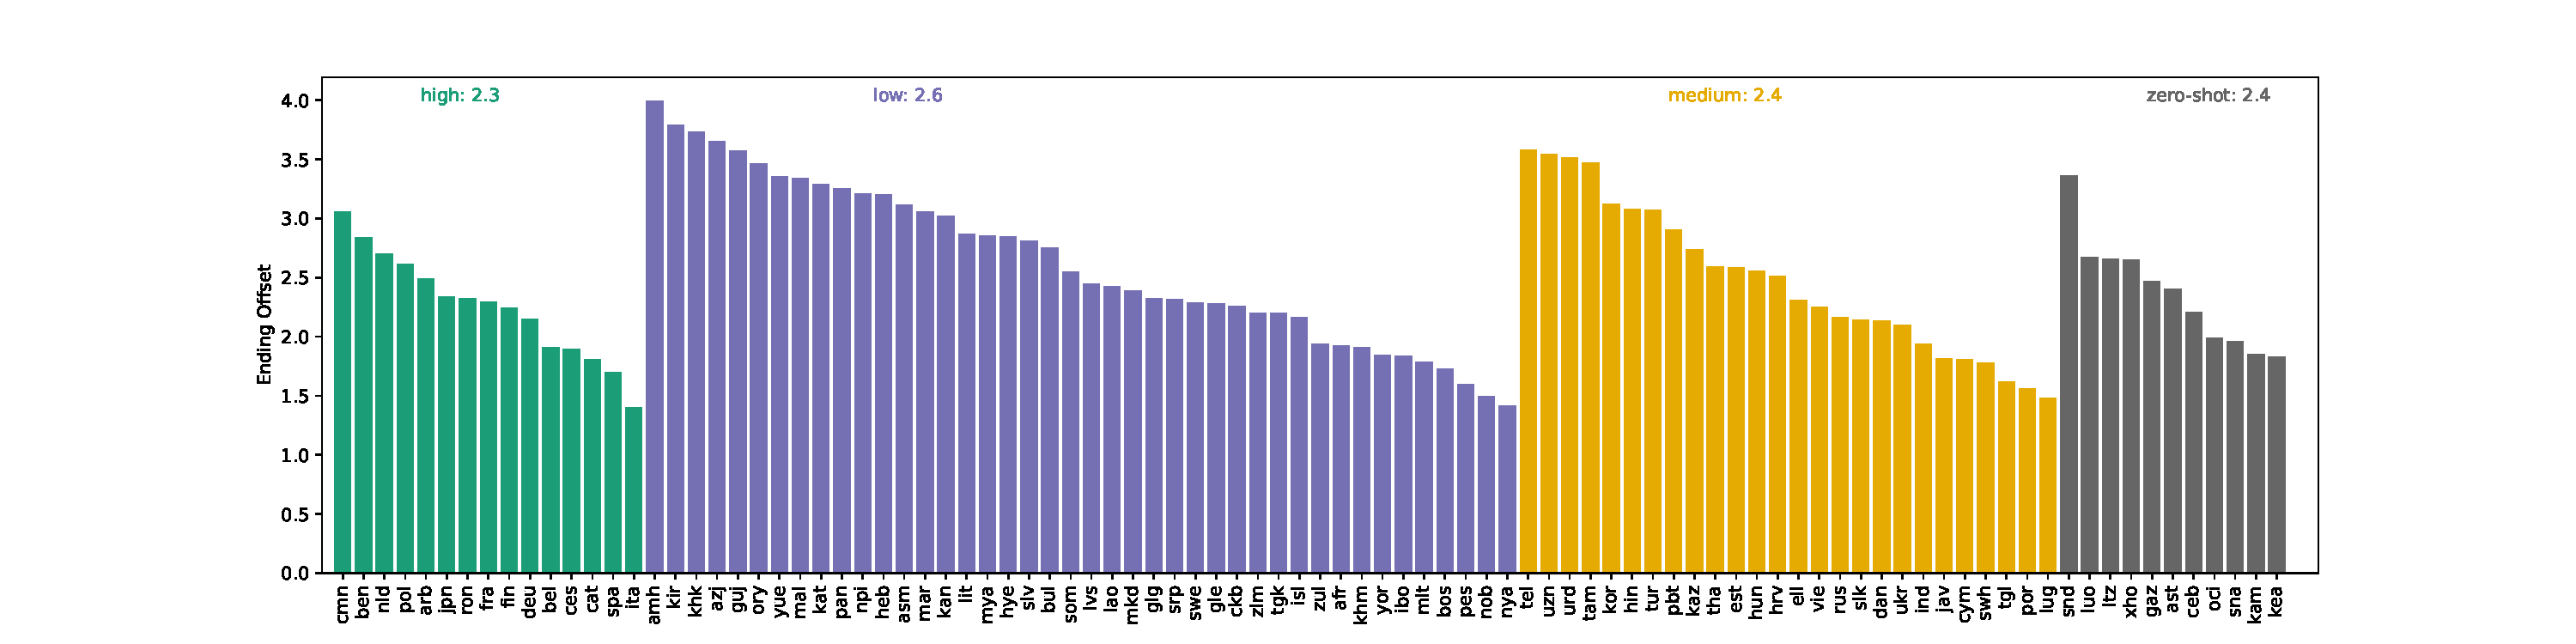
\includegraphics[width=1.0\textwidth]{figures/streaming/resources/X_ENG-EndOffset.pdf}
    \caption{Latency of \seamlessstreaming on \fleurs S2ST, \xeng.}
\end{figure}